\section{Conhecendo a Calculadora}

A Casio FX-82MS é uma calculadora científica não programável, equipada com visor de duas linhas e recursos destinados à realização de cálculos matemáticos e estatísticos. O modelo possui 240 funções, memória para nove variáveis, memória independente e recursos estatísticos, incluindo editor de dados, cálculo de desvio padrão e análise de regressão \cite{casio2004}. A alimentação é realizada por uma pilha do tipo AAA, e o equipamento possui recurso de desligamento automático para economia de energia.

\subsection{Primeira e Segunda Edição}

A segunda edição da FX-82MS representa uma atualização da linha MS com modificações principalmente relacionadas ao design, à ergonomia e à facilidade de utilização. Segundo a Casio, o projeto da segunda edição buscou proporcionar maior conforto durante o uso, melhorar a legibilidade das teclas e facilitar a identificação e o acionamento dos comandos. Entre as alterações destacadas pela fabricante estão o corpo mais arredondado, a ampliação de teclas numéricas e a utilização de caracteres mais legíveis, além de modificações na disposição e na identificação visual de algumas teclas.

\begin{figure}[H]
    \centering
    \begin{subfigure}{0.35\textwidth}
        \centering
        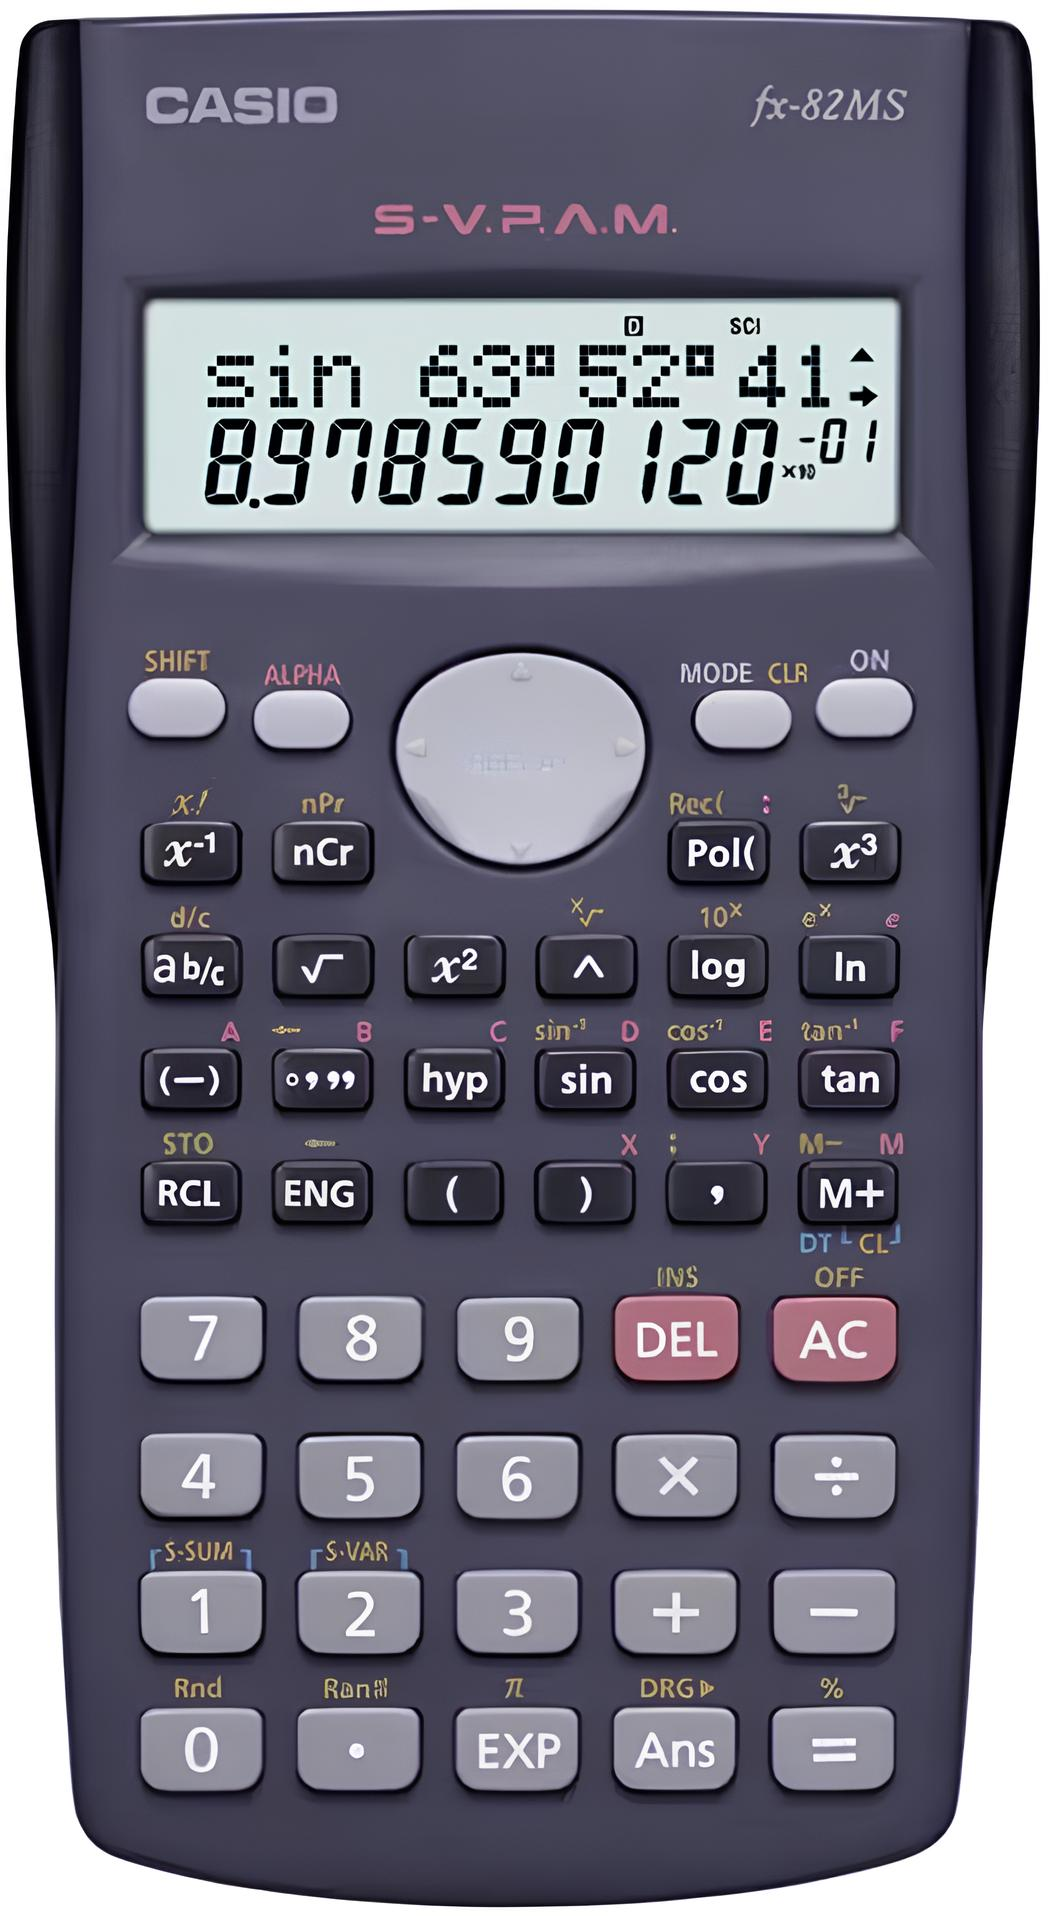
\includegraphics[width=0.66\textwidth]{img/casio-1ed.jpg}
        \caption{1\textsuperscript{a} Edição}
        \label{fig:ed1}
    \end{subfigure}
    %\hfill
    \begin{subfigure}{0.35\textwidth}
        \centering
        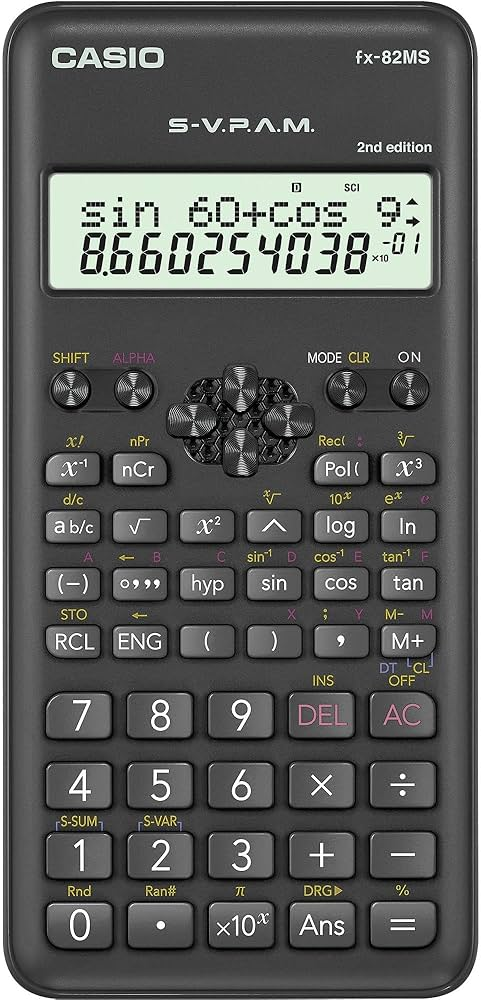
\includegraphics[width=0.58\textwidth]{img/casio-2ed.jpg}
        \caption{2\textsuperscript{a} Edição}
        \label{fig:ed2}
    \end{subfigure}
    \caption{Casio FX-82MS -- Edições}
\end{figure}

Apesar das alterações de projeto, as principais características funcionais da FX-82MS foram mantidas na segunda edição. Dessa forma, as diferenças apresentadas neste manual estão relacionadas principalmente à identificação visual e à disposição física dos elementos, e não à mudança do conteúdo estatístico abordado.

\subsection{Visor}

O visor da FX-82MS é composto por duas linhas: a linha superior exibe a 
expressão inserida pelo usuário, permitindo a conferência da entrada antes 
do cálculo, enquanto a linha inferior apresenta o resultado obtido. No topo 
do visor, pequenos indicadores informam o estado atual da calculadora:

\begin{itemize}
    \item \textbf{DEG / RAD / GRA} -- indica a unidade angular ativa para 
    cálculos trigonométricos;
    \item \textbf{M} -- indica que há um valor armazenado na memória 
    independente;
    \item \textbf{S} -- indica que a tecla \textbf{SHIFT} foi pressionada 
    e a próxima tecla ativará sua função secundária;
    \item \textbf{A} -- indica que a tecla \textbf{ALPHA} foi pressionada 
    e a próxima tecla ativará sua função terciária.
\end{itemize}

Esses indicadores são particularmente importantes durante a utilização dos recursos estatísticos e das funções acessadas por meio das teclas \textbf{SHIFT} e \textbf{ALPHA}, pois permitem identificar o estado atual da calculadora antes da execução de uma operação \cite{casio2004}.

\subsection{Teclado}

O teclado da FX-82MS é organizado de forma a concentrar múltiplas funções 
em cada tecla, reduzindo o tamanho físico do equipamento sem perda de 
funcionalidade. Cada tecla pode ter até três funções distintas:

\begin{itemize}
    \item \textbf{Função primária} -- indicada diretamente sobre a tecla, 
    ativada com um único pressionamento;
    \item \textbf{Função secundária} -- indicada em amarelo acima da tecla, 
    ativada pressionando \textbf{SHIFT} antes da tecla desejada;
    \item \textbf{Função terciária} -- indicada em vermelho acima da tecla, 
    ativada pressionando \textbf{ALPHA} antes da tecla desejada.
\end{itemize}

A identificação por cores permite localizar visualmente as funções disponíveis e compreender a sequência de teclas necessária para acessá-las \cite{casio2004}.

\subsection{Modos de Operação}

A FX-82MS oferece diferentes modos de operação, selecionados por meio da 
tecla \textbf{MODE}. A escolha do modo correto é fundamental para obter 
resultados esperados, pois cada modo altera o comportamento de diversas 
funções da calculadora:

\begin{itemize}
    \item \textbf{COMP (MODE 1)} -- modo de cálculo geral, utilizado para 
    operações aritméticas, trigonométricas, logarítmicas e demais cálculos 
    do dia a dia. É o modo padrão da calculadora;
    \item \textbf{SD (MODE 2)} -- modo de estatística com uma variável, 
    utilizado para cálculo de média, desvio padrão e soma de dados;
    \item \textbf{REG (MODE 3)} -- modo de regressão estatística, utilizado 
    para análise de correlação entre duas variáveis.
\end{itemize}

Para retornar ao modo padrão a qualquer momento, pressione \textbf{MODE}, 
em seguida \textbf{1}. Recomenda-se verificar o modo ativo antes de iniciar 
qualquer cálculo, especialmente após o uso das funções estatísticas.

\subsection{Ligando, Desligando e Reiniciando}

Para ligar a calculadora, pressione a tecla \textbf{ON}. Para desligá-la, pressione \textbf{SHIFT} seguido de \textbf{AC} (função \textbf{OFF}). A calculadora também possui um mecanismo de desligamento automático após um período sem utilização, contribuindo para a economia da bateria \cite{casio2004}.

O desligamento da calculadora não apaga os valores armazenados nas memórias. A Casio informa que a memória independente e os conteúdos das variáveis permanecem armazenados mesmo quando a calculadora é desligada \cite{casio2004}. Portanto, desligar e ligar novamente o equipamento não deve ser tratado como um procedimento de reinicialização das configurações.

Quando for necessário restaurar as configurações do modo de cálculo e de outras configurações, utilize a função \textbf{CLR}. O procedimento é:

\begin{itemize}
\item \textbf{SHIFT} $\rightarrow$ \textbf{CLR} $\rightarrow$ \textbf{2 (Mode)} -- restaura as configurações do modo de cálculo e da unidade angular para os valores iniciais;
\item \textbf{SHIFT} $\rightarrow$ \textbf{CLR} $\rightarrow$ \textbf{1 (Mcl)} -- limpa os conteúdos das memórias;
\item \textbf{SHIFT} $\rightarrow$ \textbf{CLR} $\rightarrow$ \textbf{3 (All)} -- restaura completamente a calculadora, apagando os dados armazenados e retornando as configurações aos valores iniciais.
\end{itemize}

A inicialização completa deve ser utilizada com cautela, pois remove os dados armazenados na memória da calculadora \cite{casio2004}.